% Provenance (never printed): old premiere S material on the structure of the
% Earth from seismology (P and S waves, travel times, the Moho, the shadow zone
% and the core, a reference model); see sources/book2/PROVENANCE.md. Profiles
% from figdata/grade-11/prem_profiles.py, rays and travel times from
% seismic_rays.py, the refraction lines and the problem's readings from
% moho_refraction.py. Lehmann's story and portrait are told in Book 1 (g6
% inside-the-earth): recalled here, not repeated.
\chapter{Seismische golven onthullen het binnenste}\label{ch:g11:seismic-structure}

Op 8 oktober 1909 deed een aardbeving het dal van de rivier de Kupa schudden,
ongeveer \qty{40}{km} ten zuidoosten van Zagreb, in Kroatië. Een paar maanden
eerder had Andrija Mohorovičić een nieuwe seismograaf geïnstalleerd in het
Meteorologisch Observatorium van Zagreb, en die registreerde de hele gebeurtenis.
Daarna vroeg hij andere observatoria om hun registraties en verzamelde hij die
van 41 stations. Op de registraties van de verder gelegen stations vond hij iets
onverwachts: twee afzonderlijke \omterm{def:g11:seismic-structure:body-waves}{P-golven}, een zwakke en daarna een sterkere, waar
er één had moeten zijn. Uit dat paar golven leidde hij af dat het gesteente onder
de korst anders is, en hij mat de diepte van de grens. Dit hoofdstuk laat zien hoe
de tijdstippen waarop aardbevingsgolven aankomen de lagen van de Aarde onthullen:
de onderkant van de korst, de kern en haar vloeibare buitendeel, en het hele
binnenste, diepte na diepte.
% ledger: herak:kupa-1909, srl:mohorovicic, geotech:moho-1909, kayal:pn-sn

\begin{recall}
Een aardbeving begint in een punt binnen de Aarde, de haard; het punt van het
oppervlak recht erboven is het epicentrum. Een seismometer registreert het
schudden van de grond, en de magnitude meet de grootte van een aardbeving (Boek 1,
jaar 7). De Aarde heeft een aardkorst, een mantel en een kern; de kern heeft een
vloeibaar buitendeel en een vast binnendeel. Aardbevingsgolven zijn er in twee
hoofdsoorten, de snellere \omterm{def:g11:seismic-structure:body-waves}{P-golven} en de tragere \omterm{def:g11:seismic-structure:body-waves}{S-golven}, en \omterm{def:g11:seismic-structure:body-waves}{S-golven} kunnen geen
vloeistof doorkruisen (Boek 1, jaar 6). Een golf die de grens tussen twee
materialen oversteekt waarin hij zich voortplant met de snelheden $v_1$ en $v_2$,
wordt gebroken: $\sin i_1/v_1 = \sin i_2/v_2$, waarbij de hoeken worden gemeten
ten opzichte van de loodlijn op de grens (de brekingswet van Snellius; de
natuurkundeboeken).
\end{recall}

\section{Seismische golven en looptijden}

\subsection{Twee soorten ruimtegolven}

Een aardbeving zendt golven in alle richtingen uit. Sommige lopen langs het
oppervlak; andere, de ruimtegolven, gaan door het binnenste van de Aarde, en zij
zijn het die het binnenste onthullen.

\begin{definition}[P-golf; S-golf]\label{def:g11:seismic-structure:body-waves}
Een \emph{P-golf}\index{P-golf} is een seismische golf die het gesteente
afwisselend samendrukt en uitrekt: het gesteente beweegt heen en weer langs de
richting waarin de golf zich voortplant. Ze gaat door vaste stoffen, vloeistoffen
en gassen, en is de snelste seismische golf, dus ze komt als eerste aan. Een
\emph{S-golf}\index{S-golf} vervormt het gesteente door afschuiving: het gesteente
beweegt loodrecht op de richting waarin de golf zich voortplant. Ze gaat alleen
door vaste stoffen, en komt na de P-golf aan.
\end{definition}
% ledger: kayal:p-s

Een vloeistof stroomt en biedt geen weerstand tegen een vormverandering, dus ze kan
een afschuiving niet doorgeven: daarom stoppen \omterm{def:g11:seismic-structure:body-waves}{S-golven} aan het oppervlak van een
vloeistof. In de meeste gesteenten plant een \omterm{def:g11:seismic-structure:body-waves}{P-golf} zich ongeveer
$\sqrt 3 \approx 1.7$ keer zo snel voort als een \omterm{def:g11:seismic-structure:body-waves}{S-golf}. In de bovenkorst gaat een
\omterm{def:g11:seismic-structure:body-waves}{P-golf} met ongeveer \qty{5.8}{km/s} en een \omterm{def:g11:seismic-structure:body-waves}{S-golf} met ongeveer \qty{3.2}{km/s};
vlak onder de korst bereiken ze ongeveer \qty{8.1}{km/s} en \qty{4.5}{km/s}.
% ledger: kayal:p-s, kayal:outer-core-liquid, data:prem (vp_surface 5.8, vs_surface 3.2,
% vp_upper_mantle 8.11, vs_upper_mantle 4.49 in figdata/grade-11/prem_profiles.py)

\begin{omfigure}

\includegraphics[width=0.5\linewidth]{images/book2/g11-usgs-seismometer.jpg}

{\small Seismologen van het Puerto Rico Seismic Network en van de USGS
installeren op 10 januari 2020 een tijdelijke seismometer in het zuidwesten van
Puerto Rico. Foto: Thomas Pratt, USGS (publiek domein).}
\end{omfigure}
% ledger: photo:g11-seismometer

\subsection{Looptijdkrommen}

De afstand van een aardbeving tot een ver station wordt als een hoek gemeten: de
hoek $\Delta$ in het middelpunt van de Aarde tussen het epicentrum en het station,
de \emph{epicentrale afstand}\index{epicentrale afstand}. Eén graad daarvan is
$\qty{111.2}{km}$ langs het oppervlak.
% ledger: earth:Rmean

\begin{definition}[Looptijd; looptijdkromme]\label{def:g11:seismic-structure:travel-time}
De \emph{looptijd}\index{looptijd} van een seismische golf bij een station is de
tijd die de golf nodig heeft om van de haard naar het station te gaan. De
\emph{looptijdkromme}\index{looptijdkromme} van een golf is de grafiek van haar
looptijd tegen de epicentrale afstand van het station.
\end{definition}

Een station registreert het tijdstip waarop elke golf aankomt; als het tijdstip
van de aardbeving bekend is, is het verschil de \omterm{def:g11:seismic-structure:travel-time}{looptijd}. Duizenden aardbevingen,
geregistreerd door duizenden stations, hebben de \omterm{def:g11:seismic-structure:travel-time}{looptijdkrommen} heel precies
opgeleverd. In de figuur zijn de krommen berekend met het \omterm{def:g11:seismic-structure:reference-model}{referentiemodel van de
Aarde} van \cref{sec:g11:seismic-structure:model}, en de punten zijn \omterm{def:g11:seismic-structure:travel-time}{looptijden}
die bij echte aardbevingen zijn waargenomen: de twee komen overal tot op twee
procent overeen, en meestal tot op een of twee seconden.

\begin{omfigure}
\begin{tikzpicture}
\begin{axis}[omrecord, width=0.84\linewidth, height=6.4cm, xmin=0, xmax=180, ymin=0, ymax=30,
  xtick={0,20,...,180}, ytick={0,5,...,30},
  xlabel={epicentrale afstand $\Delta$ (graden)}, ylabel={looptijd (minuten)},
  tick label style={font=\small}, label style={font=\small}, clip=false]
% computed in figdata/grade-11/seismic_rays.py; ledger: data:prem, auspass:surftim
\addplot[omDef, line width=0.9pt] table[x=delta_deg, y=t_min] {figdata/out/grade-11-seismic_rays-ttp.dat};
\addplot[omProp, line width=0.9pt] table[x=delta_deg, y=t_min] {figdata/out/grade-11-seismic_rays-tts.dat};
\addplot[omDef, line width=0.9pt, densely dashed] table[x=delta_deg, y=t_min] {figdata/out/grade-11-seismic_rays-ttpkp.dat};
\addplot[omDef!55, line width=0.9pt, densely dotted] table[x=delta_deg, y=t_min] {figdata/out/grade-11-seismic_rays-ttpkikp.dat};
\addplot[only marks, mark=*, mark size=1.5pt, black] table[x=delta_deg, y=p_min] {figdata/out/grade-11-seismic_rays-observed.dat};
\addplot[only marks, mark=*, mark size=1.5pt, black, unbounded coords=discard] table[x=delta_deg, y=s_min] {figdata/out/grade-11-seismic_rays-observed.dat};
\node[font=\small, text=omProp, anchor=south east] at (axis cs:68,21.2) {S};
\node[font=\small, text=omDef, anchor=north west] at (axis cs:72,11.2) {P};
\node[font=\small, text=omDef, anchor=south, align=center] at (axis cs:158,23.2) {P door\\de kern};
\fill[black!10] (axis cs:98.5,0) rectangle (axis cs:143.8,3.2);
\node[font=\scriptsize, align=center] at (axis cs:121.1,1.6) {geen directe P};
\end{axis}
\end{tikzpicture}

{\small \omterm{def:g11:seismic-structure:travel-time}{Looptijdkrommen} van \omterm{def:g11:seismic-structure:body-waves}{P-golven} (blauw) en \omterm{def:g11:seismic-structure:body-waves}{S-golven} (oranje) van een
aardbeving aan het oppervlak, berekend met het \omterm{def:g11:seismic-structure:reference-model}{referentiemodel van de Aarde}; de
gestreepte en gestippelde krommen zijn \omterm{def:g11:seismic-structure:body-waves}{P-golven} die door de kern zijn gegaan
(gestippeld: de binnenkern). Zwarte punten: waargenomen \omterm{def:g11:seismic-structure:travel-time}{looptijden}. Tussen
ongeveer \ang{99} en \ang{144} komt er geen \omterm{def:g11:seismic-structure:body-waves}{P-golf} rechtstreeks aan (gearceerd).}
\end{omfigure}

De S-kromme stijgt steiler dan de P-kromme, dus de vertraging tussen de twee
aankomsten groeit met de afstand. Dat geeft de afstand van een aardbeving uit één
enkele registratie.

\begin{method}[Afstand van een aardbeving uit de S--P-vertraging]\label{met:g11:seismic-structure:distance}
\begin{enumerate}
  \item Lees op de registratie het tijdstip af van de eerste \omterm{def:g11:seismic-structure:body-waves}{P-golf} en van de
        eerste \omterm{def:g11:seismic-structure:body-waves}{S-golf}; hun verschil is de S--P-vertraging.
  \item Zoek op de \omterm{def:g11:seismic-structure:travel-time}{looptijdkrommen} (of in een tabel ervan) de epicentrale afstand
        waarbij de S-kromme die vertraging boven de P-kromme
        ligt.
  \item Reken zo nodig om naar kilometer, met $\qty{111.2}{km}$ per graad.
\end{enumerate}
Met drie stations is het epicentrum het punt dat op de juiste afstand van alle
drie ligt.
\end{method}

\begin{example}[Een aardbeving op \ang{60}]\label{ex:g11:seismic-structure:sp}
Waargenomen \omterm{def:g11:seismic-structure:travel-time}{looptijden} zijn \qty{608}{s} voor P en \qty{1101}{s} voor S op
\ang{60}, \qty{536}{s} en \qty{967}{s} op \ang{50}. Een station dat een \omterm{def:g11:seismic-structure:body-waves}{S-golf}
\qty{493}{s} (8~minuten 13~seconden) na de \omterm{def:g11:seismic-structure:body-waves}{P-golf} registreert, ligt daarom
\ang{60} van het epicentrum: ongeveer $60 \times 111.2 \approx
\qty{6670}{km}$. Op \ang{50} zou de vertraging maar \qty{431}{s} zijn.
\end{example}
% ledger: auspass:surftim

\begin{omfigure}
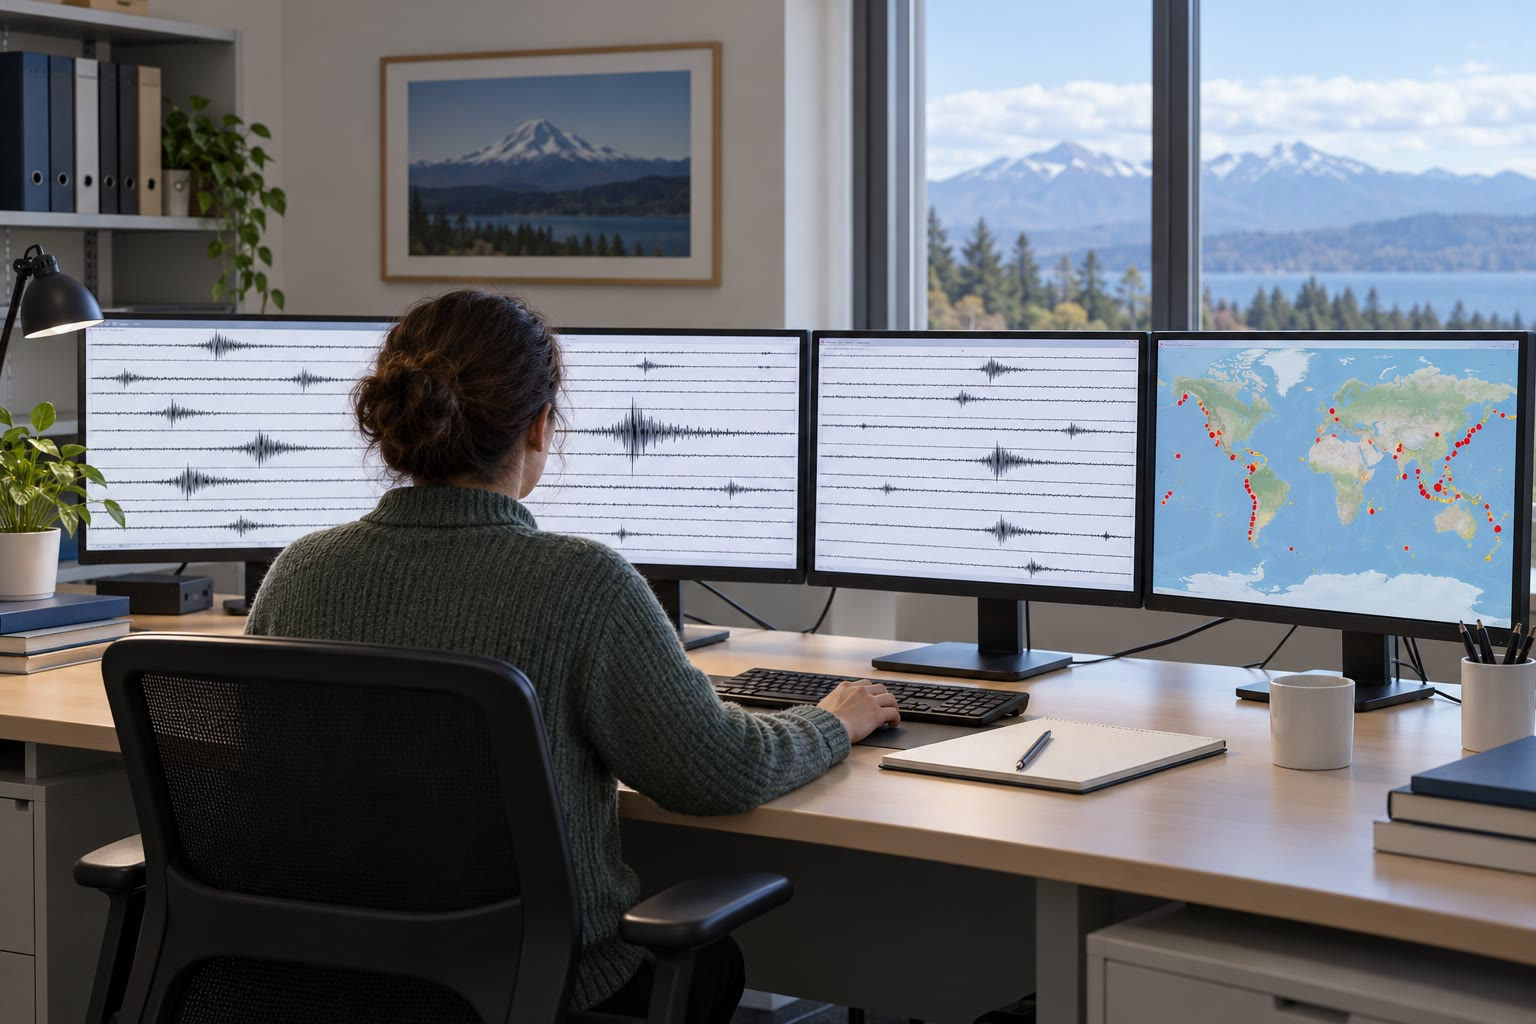
\includegraphics[width=0.66\linewidth]{images/book2/ai/g11-seismology-observatory.jpg}

{\small In een seismologisch observatorium worden de registraties van veel
stations naast elkaar getoond, en worden de aardbevingen die ze lokaliseren op een
wereldkaart uitgezet (AI-illustratie).}
\end{omfigure}

\section{Breking en de Moho}\label{sec:g11:seismic-structure:moho}

\subsection{De golf die langs een grens loopt}

In de Aarde verandert de snelheid van seismische golven met de diepte, meestal
geleidelijk, maar op sommige plaatsen ineens.

\begin{definition}[Seismische discontinuïteit]\label{def:g11:seismic-structure:discontinuity}
Een \emph{seismische discontinuïteit}\index{seismische discontinuiteit@seismische discontinuïteit} is een vlak
in de Aarde waarover de snelheid van seismische golven plotseling verandert ---
over een dikte die veel kleiner is dan de golflengte.
\end{definition}

Bij een discontinuïteit wordt een deel van een golf teruggekaatst en een deel
gebroken. Neem een laag met dikte $h$ waarin \omterm{def:g11:seismic-structure:body-waves}{P-golven} zich voortplanten met $v_1$,
boven op een laag waarin ze sneller gaan, $v_2 > v_1$. Een straal die onder de hoek
$i$ met de verticaal naar beneden gaat, wordt gebroken onder de hoek $r$ gegeven
door $\sin r = (v_2/v_1)\sin
i$: hij buigt van de verticaal af. Wanneer $\sin i$ de waarde $v_1/v_2$ bereikt,
loopt de gebroken straal precies langs de grens. De hoek
\[
  i_c, \qquad \sin i_c = \frac{v_1}{v_2},
\]
is de \emph{kritische hoek}\index{kritische hoek}. De golf die onder de \omterm{ex:g11:seismic-structure:sp}{kritische
hoek} wordt gebroken, loopt met de snelheid $v_2$ langs de bovenkant van de snellere
laag, en zendt onderweg golven terug omhoog in de bovenste laag, allemaal onder de
hoek $i_c$: die bereiken het oppervlak als de \emph{kopgolf}\index{kopgolf}.

\begin{omfigure}
\begin{tikzpicture}[x=0.05cm, y=0.05cm, font=\footnotesize, >={Stealth[length=4pt]}]
% geometry from figdata/grade-11/moho_refraction.py: v1 6.2, v2 8.1, h 30 km, ic 49.9 deg
  \fill[omLithGranite!45] (-10,0) rectangle (215,-30);
  \fill[omLithPeridotite!45] (-10,-30) rectangle (215,-48);
  \draw[line width=0.6pt] (-10,0) -- (215,0);
  \draw[line width=0.9pt] (-10,-30) -- (215,-30);
  \node[anchor=west, align=left] at (218,-15) {korst\\$v_1 = \qty{6.2}{km/s}$};
  \node[anchor=west, align=left] at (218,-39) {mantel\\$v_2 = \qty{8.1}{km/s}$};
  \node[anchor=east] at (215,-26) {Moho};
  % source and station
  \fill[omDef] (0,0) circle (1.6);
  \node[anchor=south] at (0,1.5) {aardbeving};
  \draw[fill=white] (197,0) -- (203,0) -- (200,5) -- cycle;
  \node[anchor=south] at (200,5) {station};
  % direct wave
  \draw[->, omProp, line width=0.8pt] (2,-2) -- (196,-2);
  \node[anchor=south, text=omProp] at (100,0.3) {directe golf, snelheid $v_1$};
  % head wave
  \draw[omDef, line width=0.9pt] (0,0) -- (35.7,-30);
  \draw[->, omDef, line width=0.9pt] (35.7,-30) -- (100,-30);
  \draw[omDef, line width=0.9pt] (100,-30) -- (164.3,-30) -- (200,0);
  \node[anchor=north, text=omDef] at (100,-31) {langs de Moho met $v_2$};
  \foreach \x in {50,70,90,110,130,150} {
    \draw[->, omDef!60, densely dashed] (\x,-30) -- ++(25.5,21.5);
  }
  % critical angle
  \draw[black!60, densely dotted] (35.7,-30) -- (35.7,-8);
  \draw[black!70] (35.7,-18) arc[start angle=90, end angle=130.05, radius=12];
  \node[anchor=south east] at (33,-16) {$i_c$};
  % thickness and critical distance
  \draw[<->] (-6,0) -- (-6,-30);
  \node[anchor=east] at (-7,-15) {$h$};
\end{tikzpicture}

{\small De directe golf en de \omterm{ex:g11:seismic-structure:sp}{kopgolf} (op schaal: korst \qty{30}{km} dik). De
\omterm{ex:g11:seismic-structure:sp}{kopgolf} gaat onder de \omterm{ex:g11:seismic-structure:sp}{kritische hoek} $i_c$ naar beneden, loopt langs de bovenkant
van de mantel en komt onder $i_c$ weer omhoog; over zijn hele weg langs de \omterm{def:g11:seismic-structure:moho}{Moho}
zendt hij golven naar het oppervlak (gestreept). Hij bereikt geen station dat
dichterbij ligt dan $2h\tan i_c$, hier ongeveer \qty{71}{km}.}
\end{omfigure}

\begin{proposition}[Looptijd van de kopgolf]\label{prop:g11:seismic-structure:head-wave}
Voor een bron aan het oppervlak ontvangt een station op de afstand
$x \ge 2h\tan i_c$ de \omterm{ex:g11:seismic-structure:sp}{kopgolf} na
\[
  t(x) = \frac{x}{v_2} + \frac{2h\cos i_c}{v_1}.
\]
Zijn \omterm{def:g11:seismic-structure:travel-time}{looptijdkromme} is een rechte met helling $1/v_2$ die, naar achteren
doorgetrokken, de tijdas snijdt op de \emph{intercepttijd}\index{intercepttijd}
$t_i = 2h\cos i_c/v_1$.
\end{proposition}

\begin{proof}
De straal gaat naar beneden langs een schuin stuk met lengte $h/\cos i_c$, dat
horizontaal $h\tan i_c$ vooruitgaat; omhoog doet hij hetzelfde. Daartussen loopt
hij over $x - 2h\tan i_c$ langs de grens. De tijd is
\[
  t = \frac{2h}{v_1\cos i_c} + \frac{x - 2h\tan i_c}{v_2}
    = \frac{x}{v_2} + \frac{2h}{v_1\cos i_c} - \frac{2h\sin i_c}{v_2\cos i_c}.
\]
Omdat $1/v_2 = \sin i_c/v_1$, geven de laatste twee termen samen
$\frac{2h}{v_1\cos i_c}\,(1 - \sin^2 i_c) = \frac{2h\cos i_c}{v_1}$.
\end{proof}

De directe golf komt aan na $x/v_1$: zijn kromme is een rechte door de oorsprong,
steiler dan de rechte van de \omterm{ex:g11:seismic-structure:sp}{kopgolf}. Dicht bij de bron komt de directe golf het
eerst aan; ver weg haalt de \omterm{ex:g11:seismic-structure:sp}{kopgolf}, die het grootste deel van de weg met de hogere
snelheid heeft afgelegd, hem in.

\begin{proposition}[Overgangsafstand]\label{prop:g11:seismic-structure:crossover}
De \omterm{ex:g11:seismic-structure:sp}{kopgolf} komt vóór de directe golf aan voorbij de
\emph{overgangsafstand}\index{overgangsafstand}
\[
  x_c = 2h\sqrt{\frac{v_2 + v_1}{v_2 - v_1}}.
\]
\end{proposition}

\begin{proof}
De twee komen samen aan wanneer $x/v_1 = x/v_2 + 2h\cos i_c/v_1$, dat is
$x\,(v_2 - v_1)/(v_1 v_2) = 2h\cos i_c/v_1$, dus $x = 2h\cos i_c\,v_2/(v_2 -
v_1)$. Nu is $\cos i_c = \sqrt{1 - v_1^2/v_2^2} = \sqrt{(v_2 - v_1)(v_2 +
v_1)}/v_2$, dus $x = 2h\sqrt{(v_2 + v_1)(v_2 - v_1)}/(v_2 - v_1) =
2h\sqrt{(v_2 + v_1)/(v_2 - v_1)}$. Daarvoorbij komt de \omterm{ex:g11:seismic-structure:sp}{kopgolf}, waarvan de rechte
minder steil is, het eerst aan.
\end{proof}

\begin{omfigure}
\begin{tikzpicture}
\begin{axis}[omrecord, width=0.78\linewidth, height=5.6cm, xmin=0, xmax=300, ymin=0, ymax=50,
  xtick={0,50,...,300}, xlabel={afstand tot het epicentrum (\unit{km})}, ylabel={looptijd (\unit{s})},
  tick label style={font=\small}, label style={font=\small}, clip=false]
% computed in figdata/grade-11/moho_refraction.py (critical_km 71.4, crossover_km 164.6, intercept_s 6.23)
\addplot[omProp, line width=0.9pt] table[x=x, y=tdirect] {figdata/out/grade-11-moho_refraction-model.dat};
\addplot[omDef, line width=0.9pt, restrict x to domain=71:300] table[x=x, y=thead] {figdata/out/grade-11-moho_refraction-model.dat};
\addplot[omDef, densely dashed, restrict x to domain=0:72] table[x=x, y=thead] {figdata/out/grade-11-moho_refraction-model.dat};
\draw[black!50, densely dotted] (axis cs:164.6,0) -- (axis cs:164.6,26.5);
\node[font=\scriptsize, anchor=north] at (axis cs:164.6,0) {$x_c$};
\fill (axis cs:0,6.23) circle (1.5pt);
\draw[black!60] (axis cs:0.8,6.6) -- (axis cs:6,12);
\node[font=\scriptsize, anchor=south west, inner sep=1pt] at (axis cs:5,12) {$t_i = \qty{6.2}{s}$};
\node[font=\small, text=omProp, anchor=south east] at (axis cs:250,41) {directe golf};
\node[font=\small, text=omDef, anchor=north west] at (axis cs:235,33) {kopgolf};
\end{axis}
\end{tikzpicture}

{\small \omterm{def:g11:seismic-structure:travel-time}{Looptijden} van de directe golf en van de \omterm{ex:g11:seismic-structure:sp}{kopgolf} voor de korst van de
vorige figuur. De rechte van de \omterm{ex:g11:seismic-structure:sp}{kopgolf}, naar achteren doorgetrokken
(gestreept), snijdt de tijdas op de \omterm{prop:g11:seismic-structure:head-wave}{intercepttijd}; voorbij de \omterm{prop:g11:seismic-structure:crossover}{overgangsafstand}
$x_c \approx
\qty{165}{km}$ komt de \omterm{ex:g11:seismic-structure:sp}{kopgolf} het eerst aan.}
\end{omfigure}

\subsection{De onderkant van de korst}

\begin{definition}[Moho]\label{def:g11:seismic-structure:moho}
De \emph{Mohorovičić-discontinuïteit}\index{Mohorovicic-discontinuiteit@Mohorovičić-discontinuïteit}, of
\emph{Moho}\index{Moho}, is de \omterm{def:g11:seismic-structure:discontinuity}{seismische discontinuïteit} aan de onderkant van de
korst, waar de snelheid van \omterm{def:g11:seismic-structure:body-waves}{P-golven} springt van hoogstens ongeveer \qty{7}{km/s}
naar ongeveer \qty{8}{km/s}, de snelheid in de bovenste mantel.
\end{definition}
% ledger: kayal:pn-sn, data:prem (6.8 -> 8.11 at 24.4 km)

\begin{history}[Mohorovičić en de twee P-golven, 1909]
Andrija Mohorovičić (1857--1936) vond op de registraties van de aardbeving van
1909 dat er voorbij een bepaalde afstand --- in het algemeen tussen 100 en
\qty{150}{km} --- een zwakke, snellere \omterm{def:g11:seismic-structure:body-waves}{P-golf} aankwam vóór de sterke \omterm{def:g11:seismic-structure:body-waves}{P-golf}.
Hij verklaarde die als een golf die door sneller gesteente onder de korst was
gegaan. Hij noemde de twee golven Pg (de directe golf in de korst) en Pn (de
\omterm{ex:g11:seismic-structure:sp}{kopgolf} langs de bovenkant van de mantel), deed hetzelfde voor \omterm{def:g11:seismic-structure:body-waves}{S-golven}, en leidde
de snelheden in beide lagen en de diepte van de grens ertussen af. De Pn-golf
plant zich voort met ongeveer \qty{8.0}{km/s}, de snelheid van de bovenste mantel.
Zijn artikelen van 1910 bewezen dat de korst en de mantel verschillend zijn; de
grens draagt zijn naam.
\end{history}
% ledger: kayal:pn-sn, srl:mohorovicic

\begin{method}[Diepte van de Moho uit een looptijddiagram]\label{met:g11:seismic-structure:moho}
\begin{enumerate}
  \item Zet de eerste aankomsttijden uit tegen de afstand tot het
        epicentrum.
  \item Teken de rechte van de directe golf (door de oorsprong) en de rechte
        van de \omterm{ex:g11:seismic-structure:sp}{kopgolf}; hun hellingen zijn $1/v_1$ en $1/v_2$.
  \item Trek de rechte van de \omterm{ex:g11:seismic-structure:sp}{kopgolf} naar achteren door tot de tijdas: ze snijdt
        die op de \omterm{prop:g11:seismic-structure:head-wave}{intercepttijd} $t_i$.
  \item Met $\sin i_c = v_1/v_2$ is de dikte van de korst
        $h = \dfrac{v_1\,t_i}{2\cos i_c}$.
\end{enumerate}
\end{method}

\begin{example}[Een korst van \qty{30}{km} dik]\label{ex:g11:seismic-structure:moho}
Met $v_1 = \qty{6.2}{km/s}$ en $v_2 = \qty{8.1}{km/s}$ is $\sin i_c = 0.765$,
$i_c \approx \ang{49.9}$ en $\cos i_c \approx 0.644$. Een \omterm{prop:g11:seismic-structure:head-wave}{intercepttijd} van
\qty{6.23}{s} geeft $h = 6.2 \times 6.23/(2 \times 0.644) \approx
\qty{30}{km}$. De \omterm{ex:g11:seismic-structure:sp}{kopgolf} bereikt het oppervlak voor het eerst op
$2h\tan i_c \approx \qty{71}{km}$ en haalt de directe golf in voorbij
$x_c = 60\sqrt{14.3/1.9} \approx \qty{165}{km}$.
\end{example}
% values computed in figdata/grade-11/moho_refraction.py (ic_deg 49.9, critical_km 71.4, crossover_km 164.6)

Op deze manier over de hele wereld gemeten, ligt de \omterm{def:g11:seismic-structure:moho}{Moho} maar ongeveer
\qty{5}{km} onder de bodem van de oceanen. Onder de continenten ligt hij gemiddeld
ongeveer \qty{41}{km} diep: ongeveer \qty{30}{km} waar de korst is uitgerekt,
meer dan \qty{45}{km} onder gebergtegordels, en tot ongeveer \qty{100}{km} onder
de hoogste ketens. De korst is een dun vel: zelfs \qty{41}{km} is minder dan één
procent van de straal van de Aarde.
% ledger: usgs:crust-thickness, cm95:crust, kayal:discontinuities

\section{De kern}

\subsection{Stralen die krommen}

In de mantel neemt de snelheid van seismische golven toe met de diepte. Een straal
die naar beneden gaat, doorkruist steeds sneller gesteente en wordt volgens de
brekingswet bij elke stap een beetje meer van de verticaal afgebogen: zijn baan
kromt en buigt terug naar het oppervlak. Hoe dieper een straal omkeert, hoe verder
van de aardbeving hij weer bovenkomt. De figuur toont zulke stralen, berekend met
de snelheden van het \omterm{def:g11:seismic-structure:reference-model}{referentiemodel van de Aarde}.

\begin{omfigure}
\begin{tikzpicture}
\begin{axis}[width=0.66\linewidth, height=0.66\linewidth, axis equal image, hide axis,
  xmin=-1.18, xmax=1.18, ymin=-1.18, ymax=1.2, clip=false]
% computed in figdata/grade-11/seismic_rays.py; ledger: data:prem
\fill[omLithPeridotite!25] (axis cs:0,0) circle [radius=1];
\fill[omSea!45] (axis cs:0,0) circle [radius=0.5462];
\fill[omSea!80] (axis cs:0,0) circle [radius=0.1917];
\addplot[black, line width=0.6pt, domain=0:360, samples=181] ({cos(x)}, {sin(x)});
\addplot[black!60, line width=0.4pt, domain=0:360, samples=181] ({0.5462*cos(x)}, {0.5462*sin(x)});
\addplot[black!60, line width=0.4pt, domain=0:360, samples=91] ({0.1917*cos(x)}, {0.1917*sin(x)});
\addplot[omDef, line width=0.6pt] table {figdata/out/grade-11-seismic_rays-praysmantle.dat};
\addplot[omDef!70!black, line width=0.6pt] table {figdata/out/grade-11-seismic_rays-prayscore.dat};
\addplot[omProp, line width=0.6pt] table {figdata/out/grade-11-seismic_rays-srays.dat};
% P shadow zone: 98.5 to 143.8 degrees from the source (right); S beyond 102.7 (left)
\addplot[black!80, line width=3pt, domain=-53.8:-8.5, samples=40] ({1.04*cos(x)}, {1.04*sin(x)});
\addplot[omProp!60, line width=3pt, domain=192.7:270, samples=40] ({1.04*cos(x)}, {1.04*sin(x)});
\fill[omDef] (axis cs:0,1) circle (2pt);
\node[font=\footnotesize, anchor=south] at (axis cs:0,1.04) {aardbeving};
\node[font=\footnotesize, anchor=west, align=left] at (axis cs:1.07,-0.42) {geen directe P\\(\ang{99}--\ang{144})};
\node[font=\footnotesize, anchor=east, align=right] at (axis cs:-1.07,-0.62) {geen directe S\\voorbij \ang{103}};
\node[font=\footnotesize, text=omDef, anchor=south west] at (axis cs:0.55,0.8) {P};
\node[font=\footnotesize, text=omProp, anchor=south east] at (axis cs:-0.55,0.8) {S};
\node[font=\scriptsize] at (axis cs:-0.5,-0.62) {mantel};
\node[font=\scriptsize] at (axis cs:-0.3,0.2) {buitenkern};
\draw[black!70] (axis cs:-0.1,-0.06) -- (axis cs:-0.26,-0.22);
\node[font=\scriptsize, anchor=north east, inner sep=1pt] at (axis cs:-0.24,-0.22) {binnenkern};
\end{axis}
\end{tikzpicture}

{\small Stralen van een aardbeving bovenaan de Aarde, berekend met de snelheden van
het referentiemodel. Rechts: P-stralen die in de mantel omkeren, tot ongeveer
\ang{99}, en P-stralen die door de kern gaan en voorbij ongeveer \ang{144}
uitkomen; daartussen komt geen enkele P-straal rechtstreeks aan. Links: S-stralen,
die in de mantel omkeren; geen enkele gaat door de vloeibare buitenkern, en geen
directe \omterm{def:g11:seismic-structure:body-waves}{S-golf} reikt verder dan ongeveer \ang{103}.}
\end{omfigure}

\subsection{De schaduwzone en de vloeibare buitenkern}

In 1906 merkte de seismoloog Oldham op dat \omterm{def:g11:seismic-structure:body-waves}{P-golven} die aan de andere kant van de
Aarde werden geregistreerd, later aankwamen dan verwacht, en stelde hij een
centrale kern voor waarin ze trager gaan. In 1912 toonde Gutenberg aan dat
\omterm{def:g11:seismic-structure:body-waves}{P-golven} een hele band van afstanden niet bereiken, tussen ongeveer \ang{105} en
\ang{143}, met sterke aankomsten net voorbij \ang{143}; in 1914 plaatste hij de
bovenkant van de kern op \qty{2900}{km} diepte.
% ledger: kayal:discontinuities, kayal:shadow

\begin{definition}[Schaduwzone]\label{def:g11:seismic-structure:shadow-zone}
De \emph{schaduwzone}\index{schaduwzone} van een seismische golf is het bereik van
epicentrale afstanden dat de golf vanuit een aardbeving niet rechtstreeks kan
bereiken, omdat de kern haar afbuigt of tegenhoudt.
\end{definition}

De stralen verklaren het. De P-stralen die vlak boven de kern omkeren, komen
ongeveer \ang{100} van de aardbeving weer boven. Een straal die iets steiler gaat,
komt in de kern, waar de P-snelheid plotseling daalt van \qty{13.7}{km/s} tot
ongeveer \qty{8.1}{km/s}: volgens de brekingswet buigt hij \emph{naar} de verticaal
toe, gaat door de kern en komt veel verder weg uit, voorbij ongeveer \ang{144}.
Geen enkele P-straal die in de mantel omkeert en geen enkele P-straal die door de
kern gaat, landt daartussen. In het referentiemodel loopt de \omterm{def:g11:seismic-structure:shadow-zone}{schaduwzone} van P van
\ang{98.5} tot \ang{143.8}, dicht bij de \ang{105}--\ang{143} van Gutenberg.
% ledger: kayal:shadow, data:prem (vp_above_cmb 13.72, vp_below_cmb 8.06); computed in
% figdata/grade-11/seismic_rays.py (shadow_start_deg 98.5, shadow_end_pkp_deg 143.8)

\omterm{def:g11:seismic-structure:body-waves}{S-golven} vertellen meer. Geen enkele \omterm{def:g11:seismic-structure:body-waves}{S-golf} gaat door de buitenkern: de buitenkern
geeft geen afschuifgolven door, dus ze is vloeibaar. Daardoor komt er in het
referentiemodel voorbij ongeveer \ang{103} geen enkele \omterm{def:g11:seismic-structure:body-waves}{S-golf} rechtstreeks aan ---
op de hele andere kant van de Aarde.
% ledger: kayal:outer-core-liquid; computed in figdata/grade-11/seismic_rays.py (s_direct_max_deg 102.7)

\begin{definition}[Kern-mantelgrens; grens van de binnenkern]\label{def:g11:seismic-structure:core}
De \emph{kern-mantelgrens}\index{kern-mantelgrens} is de \omterm{def:g11:seismic-structure:discontinuity}{seismische discontinuïteit}
tussen de vaste mantel en de vloeibare buitenkern, op een diepte van
\qty{2891}{km}; daar daalt de P-snelheid van ongeveer \qty{13.7}{km/s} tot
ongeveer \qty{8.1}{km/s}, en stoppen \omterm{def:g11:seismic-structure:body-waves}{S-golven}. De \emph{grens van de
binnenkern}\index{grens van de binnenkern}, op een diepte van \qty{5150}{km},
scheidt de vloeibare buitenkern van de vaste binnenkern; daar springt de
P-snelheid van ongeveer \qty{10.4}{km/s} naar ongeveer \qty{11.0}{km/s}.
\end{definition}
% ledger: data:prem, prem:cmb, prem:icb (Book 3 rows); values in figdata/grade-11/prem_profiles.py

De \omterm{def:g11:seismic-structure:shadow-zone}{schaduwzone} is niet helemaal stil: er komen zwakke \omterm{def:g11:seismic-structure:body-waves}{P-golven} in aan. Inge
Lehmann verklaarde die in 1936 met een vaste binnenkern waarin \omterm{def:g11:seismic-structure:body-waves}{P-golven} sneller
gaan (Boek 1, jaar 6). De stralen laten zien hoe. Een P-straal die de binnenkern
bereikt, buigt daar waar de snelheid omhoog springt van de verticaal af, zoals bij
de \omterm{def:g11:seismic-structure:moho}{Moho}, en komt eerder weer uit de kern: in het referentiemodel bereiken stralen
door de binnenkern het oppervlak vanaf ongeveer \ang{121}, binnen de \omterm{def:g11:seismic-structure:shadow-zone}{schaduwzone}
(gestippelde kromme van de looptijdfiguur).
% ledger: nbi:lehmann-1936 (Book 1 row), kayal:lehmann; computed in
% figdata/grade-11/seismic_rays.py (pkikp_min_deg 121.4)

\section{Een referentiemodel van de Aarde}\label{sec:g11:seismic-structure:model}

Samengevoegd geven miljoenen \omterm{def:g11:seismic-structure:travel-time}{looptijden} de snelheid van P- en \omterm{def:g11:seismic-structure:body-waves}{S-golven} op elke
diepte. Hun snelheden hangen af van het gesteente en zijn dichtheid, en de totale
massa van de Aarde legt haar gemiddelde dichtheid vast; samen geven ze ook de
dichtheid op elke diepte.
% ledger: data:prem, prem:constraints (Book 3 row)

\begin{definition}[Referentiemodel van de Aarde]\label{def:g11:seismic-structure:reference-model}
Een \emph{referentiemodel van de Aarde}\index{referentiemodel van de Aarde} is
een tabel van de snelheid van \omterm{def:g11:seismic-structure:body-waves}{P-golven}, de snelheid van \omterm{def:g11:seismic-structure:body-waves}{S-golven} en de dichtheid
tegen de diepte, in elke richting dezelfde, gekozen om overeen te komen met de
waargenomen \omterm{def:g11:seismic-structure:travel-time}{looptijden} van seismische golven en met de massa van de Aarde.
\end{definition}

Het meest gebruikte is het Preliminary Reference Earth Model (PREM), in 1981
gepubliceerd door A.~M.~Dziewonski en D.~L.~Anderson. De stralen en \omterm{def:g11:seismic-structure:travel-time}{looptijden}
van dit hoofdstuk zijn ermee berekend: de \omterm{def:g11:seismic-structure:travel-time}{looptijd} van P op \ang{60} komt
bijvoorbeeld uit op \qty{607}{s}, tegen \qty{608}{s} waargenomen.
% ledger: data:prem, auspass:surftim; computed in figdata/grade-11/seismic_rays.py (p_60_s 607.2)

\begin{omfigure}
\begin{tikzpicture}
\begin{axis}[omrecord, width=0.86\linewidth, height=6.2cm, xmin=0, xmax=6371, ymin=0, ymax=14.5,
  xtick={0,1000,...,6000}, ytick={0,2,...,14}, scaled x ticks=false,
  xticklabel style={/pgf/number format/1000 sep={\,}},
  xlabel={diepte (\unit{km})}, ylabel={snelheid (\unit{km/s}) of dichtheid (\unit{g/cm^3})},
  tick label style={font=\small}, label style={font=\small}, clip=false]
% computed in figdata/grade-11/prem_profiles.py; ledger: data:prem
\addplot[omDef, line width=0.9pt] table[x=depth, y=vp] {figdata/out/grade-11-prem_profiles-profile.dat};
\addplot[omProp, line width=0.9pt] table[x=depth, y=vs] {figdata/out/grade-11-prem_profiles-profile.dat};
\addplot[black, line width=0.9pt, densely dashed] table[x=depth, y=rho] {figdata/out/grade-11-prem_profiles-profile.dat};
\foreach \d in {670,2891,5149.5} {\edef\temp{\noexpand\draw[black!40, densely dotted] (axis cs:\d,0) -- (axis cs:\d,14.5);}\temp}
\node[font=\scriptsize, anchor=south, align=center] at (axis cs:2891,14.5) {kern-\\mantelgrens};
\node[font=\scriptsize, anchor=south, align=center] at (axis cs:5149.5,14.5) {grens van\\de binnenkern};
\node[font=\scriptsize, anchor=south] at (axis cs:670,14.5) {\qty{670}{km}};
\node[font=\small, text=omDef, anchor=south] at (axis cs:1800,12.4) {P-snelheid};
\node[font=\small, text=omProp, anchor=south] at (axis cs:1800,7.0) {S-snelheid};
\node[font=\small, anchor=north] at (axis cs:1800,4.5) {dichtheid};
\node[font=\scriptsize, align=center] at (axis cs:4000,1.9) {geen S-golven:\\vloeibaar};
\end{axis}
\end{tikzpicture}

{\small De snelheden van P- en \omterm{def:g11:seismic-structure:body-waves}{S-golven} en de dichtheid tegen de diepte in het
Preliminary Reference Earth Model (Dziewonski en Anderson, 1981). De
stippellijnen markeren de belangrijkste discontinuïteiten onder de \omterm{def:g11:seismic-structure:moho}{Moho}, die te
ondiep ligt om op deze schaal te zien.}
\end{omfigure}

Het model van boven naar beneden gelezen:
\begin{itemize}
  \item de korst, met P-snelheden van 5.8 tot \qty{6.8}{km/s}, eindigt bij de \omterm{def:g11:seismic-structure:moho}{Moho}
        (\qty{24.4}{km} in dit gemiddelde model);
  \item in de mantel nemen de snelheden toe met de diepte, met kleinere plotselinge
        sprongen, de grootste bij \qty{400}{km} en \qty{670}{km};
  \item op \qty{2891}{km} valt de S-snelheid terug tot nul en daalt de P-snelheid
        met meer dan \qty{5}{km/s}: de vloeibare buitenkern;
  \item op \qty{5150}{km} bestaan er weer \omterm{def:g11:seismic-structure:body-waves}{S-golven}: de vaste binnenkern,
        met een straal van \qty{1220}{km}.
\end{itemize}
% ledger: data:prem (discontinuities in figdata/grade-11/prem_profiles.py)

De dichtheid stijgt van \qty{2.6}{g/cm^3} in de korst tot
\qty{5.6}{g/cm^3} aan de onderkant van de mantel, springt dan naar
\qty{9.9}{g/cm^3} bovenaan de kern en bereikt \qty{13.1}{g/cm^3} in het
middelpunt. De gemiddelde dichtheid van het hele model is \qty{5.5}{g/cm^3}, twee
keer die van de gesteenten van de korst: het diepe binnenste, en vooral de kern,
bestaat uit veel dichter materiaal dan het oppervlak. De kern bevat ongeveer een
derde van de massa van de Aarde.
% ledger: data:prem, prem:cmb, prem:centre (Book 3 rows); computed in
% figdata/grade-11/prem_profiles.py (mean_density 5.52; core mass fraction 0.32)

\section{Oefeningen}

\begin{exercise}[$\star$]\label{exo:g11:seismic-structure:1}
Geef twee verschillen tussen \omterm{def:g11:seismic-structure:body-waves}{P-golven} en \omterm{def:g11:seismic-structure:body-waves}{S-golven}. Welke wordt het eerst door een
seismometer geregistreerd, en waarom?
\end{exercise}

\begin{exercise}[$\star$]\label{exo:g11:seismic-structure:2}
Een station ligt \ang{40} van een epicentrum. Hoe ver is het, gemeten langs het
oppervlak? Hoeveel graden ligt een station op \qty{8900}{km} van een epicentrum
daarvandaan?
\end{exercise}

\begin{exercise}[$\star$]\label{exo:g11:seismic-structure:3}
De waargenomen \omterm{def:g11:seismic-structure:travel-time}{looptijden} op \ang{40} zijn \qty{456}{s} voor P en
\qty{822}{s} voor S. Reken ze om naar minuten en seconden, en geef de
S--P-vertraging.
\end{exercise}

\begin{exercise}[$\star$]\label{exo:g11:seismic-structure:4}
Een korst waarin \omterm{def:g11:seismic-structure:body-waves}{P-golven} zich voortplanten met \qty{6.0}{km/s} ligt op een
mantel waar ze \qty{8.0}{km/s} halen. Bereken de \omterm{ex:g11:seismic-structure:sp}{kritische hoek}.
\end{exercise}

\begin{exercise}[$\star$]\label{exo:g11:seismic-structure:5}
In het referentiemodel ligt de \omterm{def:g11:seismic-structure:core}{kern-mantelgrens} op \qty{2891}{km} diepte en de
\omterm{def:g11:seismic-structure:core}{grens van de binnenkern} op \qty{5150}{km}; de straal van de Aarde is
\qty{6371}{km}. Bereken de dikte van de buitenkern, de straal van de kern, en de
straal van de kern als deel van de straal van de Aarde.
\end{exercise}

\begin{exercise}[$\star\star$]\label{exo:g11:seismic-structure:6}
Waargenomen S--P-vertragingen zijn \qty{224}{s} op \ang{20}, \qty{298}{s} op
\ang{30}, \qty{366}{s} op \ang{40}, \qty{431}{s} op \ang{50} en
\qty{493}{s} op \ang{60}. Een station registreert een \omterm{def:g11:seismic-structure:body-waves}{S-golf} 6~minuten 6~seconden
na de \omterm{def:g11:seismic-structure:body-waves}{P-golf}. Hoe ver weg is de aardbeving, in graden en in kilometer?
Waarom kan één station niet zeggen waar de aardbeving is?
\end{exercise}

\begin{exercise}[$\star\star$]\label{exo:g11:seismic-structure:7}
Bereken met de snelheden van \cref{exo:g11:seismic-structure:4} en een korst van
\qty{35}{km} dik de \omterm{def:g11:seismic-structure:travel-time}{looptijden} van de directe golf en van de \omterm{ex:g11:seismic-structure:sp}{kopgolf} bij een
station op \qty{200}{km} van het epicentrum. Welke komt het eerst aan?
\end{exercise}

\begin{exercise}[$\star\star$]\label{exo:g11:seismic-structure:8}
Bereken voor de korst van \cref{exo:g11:seismic-structure:7} de kritische
afstand $2h\tan i_c$ en de \omterm{prop:g11:seismic-structure:crossover}{overgangsafstand}. Ga na dat het antwoord op
\cref{exo:g11:seismic-structure:7} daarmee klopt.
\end{exercise}

\begin{exercise}[$\star\star$]\label{exo:g11:seismic-structure:9}
Onder een oceaan ligt een korst van \qty{6}{km} dik, waarin \omterm{def:g11:seismic-structure:body-waves}{P-golven} zich
voortplanten met \qty{6.5}{km/s}, op een mantel met \qty{8.0}{km/s}. Bereken de
\omterm{ex:g11:seismic-structure:sp}{kritische hoek}, de \omterm{prop:g11:seismic-structure:head-wave}{intercepttijd} en de \omterm{prop:g11:seismic-structure:crossover}{overgangsafstand}. Waarom moeten de stations
veel dichter bij elkaar staan om de \omterm{def:g11:seismic-structure:moho}{Moho} onder een oceaan te vinden dan onder een
continent?
\end{exercise}

\begin{exercise}[$\star\star$]\label{exo:g11:seismic-structure:10}
Een P-straal in de onderste mantel, waar hij zich voortplant met \qty{13.7}{km/s},
treft de \omterm{def:g11:seismic-structure:core}{kern-mantelgrens} onder \ang{30} met de loodlijn. Onder de grens is de
P-snelheid \qty{8.06}{km/s}. Bereken de hoek van de gebroken straal. Buigt de
straal naar de loodlijn toe of ervan af? Gebruik dit om uit te leggen waarom
P-stralen die de kern binnengaan, ver van de aardbeving uitkomen.
\end{exercise}

\begin{exercise}[$\star\star$]\label{exo:g11:seismic-structure:11}
In het referentiemodel doet een \omterm{def:g11:seismic-structure:body-waves}{P-golf} die recht naar beneden door het middelpunt
gaat \qty{1210}{s} over het bereiken van het tegenoverliggende punt van de Aarde.
Hoe lang zou dat duren als ze de hele middellijn (\qty{12742}{km}) met
\qty{13.7}{km/s} aflegde, de P-snelheid aan de onderkant van de mantel? Wat
concludeerde Oldham uit zulke vertragingen?
\end{exercise}

\begin{exercise}[$\star\star\star$]\label{exo:g11:seismic-structure:12}
(1) Toon met \cref{prop:g11:seismic-structure:head-wave} aan dat de dikte
van de korst gelijk is aan
\[
  h = \frac{t_i\,v_1 v_2}{2\sqrt{v_2^2 - v_1^2}}.
\]
(2) Pas dit toe op $t_i = \qty{6.23}{s}$, $v_1 = \qty{6.2}{km/s}$ en
$v_2 = \qty{8.1}{km/s}$.
\end{exercise}

\begin{exercise}[$\star\star\star$]\label{exo:g11:seismic-structure:13}
De gemiddelde dichtheid van de Aarde is \qty{5.52}{g/cm^3}. Beschouw de Aarde als
een kern met straal \qty{3480}{km} en uniforme dichtheid $\rho_c$, binnen een
mantel en korst met uniforme dichtheid \qty{4.45}{g/cm^3} (het gemiddelde van het
referentiemodel). (1) Welk deel van het volume van de Aarde is de kern? (2) Bereken
$\rho_c$. (3) Vergelijk met de dichtheid bovenaan de kern in het
referentiemodel, \qty{9.9}{g/cm^3}, en met de dichtheid van de korst.
\end{exercise}

\begin{exercise}[$\star\star\star$]\label{exo:g11:seismic-structure:14}
De \omterm{def:g11:seismic-structure:shadow-zone}{schaduwzone} van P van Gutenberg loopt van \ang{105} tot \ang{143}. (1) Geef
haar grenzen in kilometer langs het oppervlak. (2) Op een bol is het oppervlak
tussen de hoekafstanden $a$ en $b$ van een punt het deel $(\cos a - \cos
b)/2$ van het hele oppervlak. Welk deel van het aardoppervlak ontvangt geen directe
\omterm{def:g11:seismic-structure:body-waves}{P-golf} van een gegeven aardbeving? (3) Waarom heeft elke aardbeving haar eigen
\omterm{def:g11:seismic-structure:shadow-zone}{schaduwzone}?
\end{exercise}

\begin{exercise}[$\star\star\star$]\label{exo:g11:seismic-structure:15}
Onder een hoge bergketen vindt een refractieonderzoek $v_1 =
\qty{6.3}{km/s}$, $v_2 = \qty{8.1}{km/s}$ en een \omterm{prop:g11:seismic-structure:head-wave}{intercepttijd} van
\qty{9.5}{s}. (1) Bereken daar de dikte van de korst. (2) Welke \omterm{prop:g11:seismic-structure:head-wave}{intercepttijd} zou
een korst van \qty{30}{km} dik met dezelfde snelheden geven?
(3) Vergelijk met de gemiddelde dikte van de continentale korst.
\end{exercise}

\section{Probleem: de Moho vinden}

\begin{problem}[{Weekendprobleem --- de dikte van de korst uit vijftien stations}]
\label{pb:g11:seismic-structure:1}
% readings computed in figdata/grade-11/moho_refraction.py (part stations; invented region,
% v1 6.2, v2 8.1, h 30 km, reading errors of up to 0.1 s); ledger: kayal:pn-sn, usgs:crust-thickness
Een kleine aardbeving vindt op heel geringe diepte onder een continent plaats.
Vijftien stations, opgesteld op een rechte lijn vanaf het epicentrum, registreren
de aankomsttijden van de eerste \omterm{def:g11:seismic-structure:body-waves}{P-golf} en, waar die af te lezen is, van een tweede.
De aflezingen hieronder zijn verzonnen, maar berekend zoals een echt onderzoek ze
zou vinden, tot op een tiende seconde. Pg is de golf die door de korst gaat, Pn de
golf die langs de bovenkant van de mantel is gelopen.

\begin{center}
\small
\begin{tabular}{|c|c|c||c|c|c|}
\hline
afstand (\unit{km}) & Pg (\unit{s}) & Pn (\unit{s}) & afstand (\unit{km}) & Pg (\unit{s}) & Pn (\unit{s}) \\ \hline
20 & 3.3 & --- & 180 & 29.0 & 28.5 \\ \hline
40 & 6.5 & --- & 200 & 32.3 & 30.9 \\ \hline
60 & 9.7 & --- & 220 & --- & 33.3 \\ \hline
80 & 12.8 & 16.2 & 240 & --- & 35.8 \\ \hline
100 & 16.1 & 18.6 & 260 & --- & 38.3 \\ \hline
120 & 19.3 & 21.1 & 280 & --- & 40.8 \\ \hline
140 & 22.6 & 23.6 & 300 & --- & 43.2 \\ \hline
160 & 25.8 & 26.0 & & & \\ \hline
\end{tabular}
\end{center}

\medskip
\noindent\textbf{Deel I --- De directe golf.}
\begin{enumerate}
  \item Zet op millimeterpapier de tijden van Pg en Pn uit tegen de afstand
        (\qty{1}{cm} voor \qty{20}{km} en voor \qty{5}{s}). Hoe liggen de punten van Pg?
  \item Waarom gaat de rechte van Pg dicht langs de oorsprong?
  \item Bereken met de stations op 20 en \qty{200}{km} de helling van de
        rechte van Pg in seconde per kilometer.
  \item Leid daaruit de snelheid $v_1$ van \omterm{def:g11:seismic-structure:body-waves}{P-golven} in de korst af.
  \item Als de korst doorliep, wanneer zou de Pg-golf dan het station op
        \qty{300}{km} bereiken?
\end{enumerate}

\medskip
\noindent\textbf{Deel II --- De gebroken golf.}
\begin{enumerate}[resume]
  \item Bereken met de stations op 100 en \qty{300}{km} de helling van de
        rechte van Pn en de snelheid $v_2$ van \omterm{def:g11:seismic-structure:body-waves}{P-golven} onder de korst.
  \item Vergelijk $v_2$ met de snelheid van de Pn-golf die Mohorovičić mat,
        ongeveer \qty{8.0}{km/s}. Welk gesteente ligt onder de korst?
  \item Bereken de \omterm{ex:g11:seismic-structure:sp}{kritische hoek} $i_c$.
  \item Geen enkel station dichter dan \qty{80}{km} registreert een Pn-golf. Leg
        met \cref{prop:g11:seismic-structure:head-wave} uit waarom er een
        kleinste afstand is waarop de \omterm{ex:g11:seismic-structure:sp}{kopgolf} kan worden geregistreerd.
  \item Tussen 80 en \qty{160}{km} komt Pn na Pg aan. Waarom wordt ze toch
        geregistreerd?
\end{enumerate}

\medskip
\noindent\textbf{Deel III --- De overgang.}
\begin{enumerate}[resume]
  \item Tussen welke twee stations verandert volgens de tabel de eerst aankomende
        golf van Pg in Pn?
  \item Schrijf de vergelijkingen van de twee rechten op, met de punten op
        \qty{20}{km} (Pg) en \qty{100}{km} (Pn).
  \item Bereken de afstand waarop de twee rechten elkaar snijden.
  \item Voorbij \qty{200}{km} registreert geen enkel station Pg als een
        afzonderlijke golf. Welke golf registreert een station op \qty{250}{km}
        het eerst, en wanneer?
\end{enumerate}

\medskip
\noindent\textbf{Deel IV --- De diepte van de Moho.}
\begin{enumerate}[resume]
  \item Trek de rechte van Pn naar achteren door tot de tijdas: wat is de
        \omterm{prop:g11:seismic-structure:head-wave}{intercepttijd} $t_i$?
  \item Bereken $\cos i_c$, en de dikte $h$ van de korst met
        \cref{met:g11:seismic-structure:moho}.
  \item Controle: bereken met deze $h$ de \omterm{prop:g11:seismic-structure:crossover}{overgangsafstand} met
        \cref{prop:g11:seismic-structure:crossover} en vergelijk met
        vraag~13.
  \item Nog een controle: bereken de kritische afstand $2h\tan i_c$ en vergelijk
        met het dichtstbijzijnde station dat Pn registreert.
  \item De seismologen geven $h$ maar tot op een paar kilometer. Waarom is een
        nauwkeuriger waarde niet gerechtvaardigd?
  \item Besluit: op welke diepte ligt de \omterm{def:g11:seismic-structure:moho}{Moho} onder dit gebied? Is de korst hier
        dun of dik voor een continent?
\end{enumerate}
\end{problem}
